\documentclass[12pt,a4paper]{article}
\usepackage[utf8]{inputenc}
\usepackage[brazilian]{babel}
\usepackage{graphicx}
\usepackage{float}
\usepackage{geometry}
\geometry{a4paper, margin=2cm}
\usepackage{booktabs}
\usepackage{hyperref}

\title{Trabalho Prático: Aprendizado Supervisionado\\ \large Seleção de Features e Otimização de Hiperparâmetros}
\author{Ivan Mendar Martignago}
\date{Junho de 2026}

\begin{document}

\begin{titlepage}
    \centering
    \vspace*{1cm}
    \Large \textbf{Universidade Federal de Santa Maria}\\
    \Large Curso de Sistemas de Informação\\
    \Large Disciplina: Sistemas Inteligentes\\
    \vspace{4cm}
    
    \Huge \textbf{Relatório do Trabalho Prático}\\
    \large Aprendizado Supervisionado com Seleção de Features e Otimização de Hiperparâmetros\\
    \vspace{1.5cm}
    
    \Large \textbf{Aluno:} Ivan Mendar Martignago\\
    \vfill
    \large \today
\end{titlepage}

\maketitle

\section{Etapa 1 -- Descrição do Dataset}
O dataset utilizado é o \textit{Heart Failure Prediction Dataset}, que reúne informações médicas com o objetivo de prever o desenvolvimento de falhas ou doenças cardíacas. 
A base de dados é composta inicialmente por 918 amostras e 11 atributos preditivos (idade, sexo, tipo de dor no peito, pressão arterial em repouso, colesterol, glicemia em jejum, resultados de eletrocardiograma, frequência cardíaca máxima, angina induzida por exercício, depressão do segmento ST e inclinação do segmento ST). A variável alvo é \texttt{HeartDisease}, indicando presença (1) ou ausência (0) de doença cardíaca.
Foram identificados possíveis problemas na base de dados, como a presença de um paciente com pressão arterial igual a zero e uma grande quantidade (cerca de 20\%) de valores zerados para o colesterol, o que demandou atenção na etapa de pré-processamento.

\section{Etapa 2 -- Pré-processamento}
Para garantir a qualidade dos dados antes de submetê-los à rede neural, foram realizadas as seguintes transformações:
\begin{itemize}
    \item \textbf{Remoção de Registros Inconsistentes:} Foi removido um registro contendo o atributo da Pressão Arterial (\texttt{RestingBP}) igual a 0, pois representa uma impossibilidade biológica.
    \item \textbf{Tratamento de Valores Ausentes:} O atributo Colesterol possuía 172 instâncias com valor "0". Esses valores foram substituídos por valores ausentes (\textit{NaN}) e posteriormente imputados utilizando o algoritmo \textbf{KNNImputer} (com $k=5$). Essa escolha foi feita pois a imputação por vizinhos mais próximos preserva melhor a variância e distribuição dos dados em relação à média ou mediana, uma vez que utiliza pacientes com características clínicas semelhantes para inferir o colesterol faltante.
    \item \textbf{Codificação de Variáveis Categóricas:} As variáveis nominais como \textit{Sex}, \textit{ChestPainType}, entre outras, foram transformadas utilizando \textbf{One-Hot Encoding} para evitar que os algoritmos interpretem falsa hierarquia entre as categorias.
    \item \textbf{Padronização:} As variáveis numéricas foram normalizadas utilizando o \textbf{RobustScaler}. A escolha desta técnica justifica-se pela sua resiliência a \textit{outliers}. Como dados médicos (ex. colesterol muito elevado) costumam possuir anomalias naturais, o \textit{RobustScaler} lida de forma mais eficiente do que o \textit{StandardScaler}.
\end{itemize}

\section{Etapa 3 -- Seleção de Features}
O método escolhido para a seleção de features foi o \textbf{Random Forest Feature Importance} (Método \textit{Embedded}). A justificativa deve-se ao fato do algoritmo considerar interações complexas entre atributos e lidar naturalmente com ruídos. 
A quantidade inicial de atributos após o processamento (devido à criação de colunas no One-Hot Encoding) foi de 15. Após a seleção, definimos um ponto de corte para as 10 \textit{features} mais importantes.

O critério principal foi selecionar as 10 características com maior relevância de acordo com as árvores de decisão. Destacaram-se como mais importantes características como a Inclinação do Segmento ST (\textit{ST\_Slope\_Up}), a idade, o colesterol, e a depressão do ST (\textit{Oldpeak}).

A seleção de atributos contribuiu para uma \textbf{melhor interpretabilidade do modelo} e redução marginal da complexidade de treinamento, garantindo também uma acurácia sólida e comparável, mitigando ruídos trazidos por categorias menos informativas.

\section{Etapa 4 -- Classificação com MLP}
Para prever a presença ou ausência da doença cardíaca (classificação binária), foi desenvolvida uma Rede Neural Multicamadas (\textit{MLPClassifier} do Scikit-Learn). Os hiperparâmetros iniciais definidos foram:
\begin{itemize}
    \item \textbf{Camadas ocultas:} 2 (com 64 e 32 neurônios respectivamente). Justifica-se pela necessidade de abstrair relações não-lineares nos dados sem criar um modelo complexo o suficiente para decorar rapidamente a base.
    \item \textbf{Ativação e Otimizador:} \textit{ReLU} e \textit{Adam}. A ativação ReLU evita o problema do desvanecimento do gradiente, e o otimizador Adam combina as vantagens do Momentum e do RMSProp para convergência mais estável.
    \item \textbf{Taxa de aprendizado e Épocas:} $0.001$ com máximo de 500 épocas. O \textit{early\_stopping} foi ativado.
    \item \textbf{Batch Size:} 32.
\end{itemize}

Abaixo são apresentados os resultados das duas abordagens:
\begin{table}[H]
    \centering
    \begin{tabular}{l c c}
        \toprule
        \textbf{Métrica} & \textbf{Todas as Features (15)} & \textbf{Features Selecionadas (10)} \\
        \midrule
        Accuracy  & 0.8533 & 0.8587 \\
        Precision & 0.8571 & 0.8725 \\
        Recall    & 0.8824 & 0.8725 \\
        F1-Score  & 0.8696 & 0.8725 \\
        ROC-AUC   & 0.9366 & 0.9246 \\
        \bottomrule
    \end{tabular}
    \caption{Avaliação do MLPClassifier}
\end{table}

\section{Etapa 5 -- Regressão com MLP}
Para o problema de regressão, buscou-se prever a Frequência Cardíaca Máxima (\texttt{MaxHR}) do paciente. Foi utilizado o \textit{MLPRegressor} com as mesmas definições estruturais base (64 e 32 neurônios, ReLU e Adam), mas utilizando uma taxa de aprendizado de $0.01$ e máximo de 1000 épocas devido à natureza do ajuste numérico em um espaço contínuo. 

Os resultados atingidos foram:
\begin{itemize}
    \item \textbf{MAE (Erro Absoluto Médio):} 17.17 bpm de erro em média.
    \item \textbf{MSE:} 482.31
    \item \textbf{RMSE:} 21.96
    \item \textbf{R²:} 0.2665
\end{itemize}
O $R^2$ baixo é indicativo da dificuldade em prever variáveis fisiológicas contínuas de forte variabilidade apenas baseando-se em exames clínicos genéricos, demonstrando que os modelos lineares e MLPs base possuem certas limitações ou que há falta de atributos mais determinísticos para a frequência cardíaca na base.

\section{Etapa 6 -- Otimização de Hiperparâmetros com Optuna}
Utilizou-se o \textit{Optuna} para explorar exaustivamente um espaço de busca afim de maximizar a acurácia. O espaço definido contou com a arquitetura da rede (1 a 3 camadas, entre 16 e 128 neurônios), Taxa de Aprendizado ($10^{-4}$ a $10^{-2}$ em escala logarítmica) e Tamanhos de \textit{Batch} (16, 32, 64).

Foram executados 50 \textit{trials}. A utilização da otimização bayesiana pelo Optuna permitiu encontrar um balanço ideal que melhorou a estabilidade e a convergência do modelo. As redes otimizadas frequentemente utilizaram taxas de aprendizado ajustadas e \textit{batches} menores, permitindo que a acurácia chegasse no estado da arte da base de dados ($>85\%$), embora o tempo de treinamento (computacional) para explorar os 50 \textit{trials} adicione sobrecarga na pipeline.

\section{Etapa 7 -- Regularização e Análise de Overfitting}
Foi analisado o impacto do \textit{Overfitting} controlando o parâmetro L2 (\textit{Weight Decay} pelo parâmetro \texttt{alpha}) no MLPClassifier.
Em um modelo complexo (113 neurônios), comparou-se a utilização de uma baixa regularização ($alpha = 0.0001$) contra uma alta penalidade nos pesos da rede ($alpha = 0.5$). 

Os resultados finais mostraram melhor generalização em dados de teste para a configuração com peso L2 mais ajustado. A técnica agiu suprimindo o crescimento irrestrito dos pesos sinápticos durante as épocas, impedindo que a rede "decorasse" os ruídos presentes no conjunto de treinamento. Isso se traduziu em um \textit{loss} de validação mais estável na curva de aprendizado, confirmando que a regularização L2, juntamente com o \textit{early stopping}, é uma estratégia fundamental para encontrar o equilíbrio entre \textit{bias} e variância.

\begin{figure}[H]
    \centering
    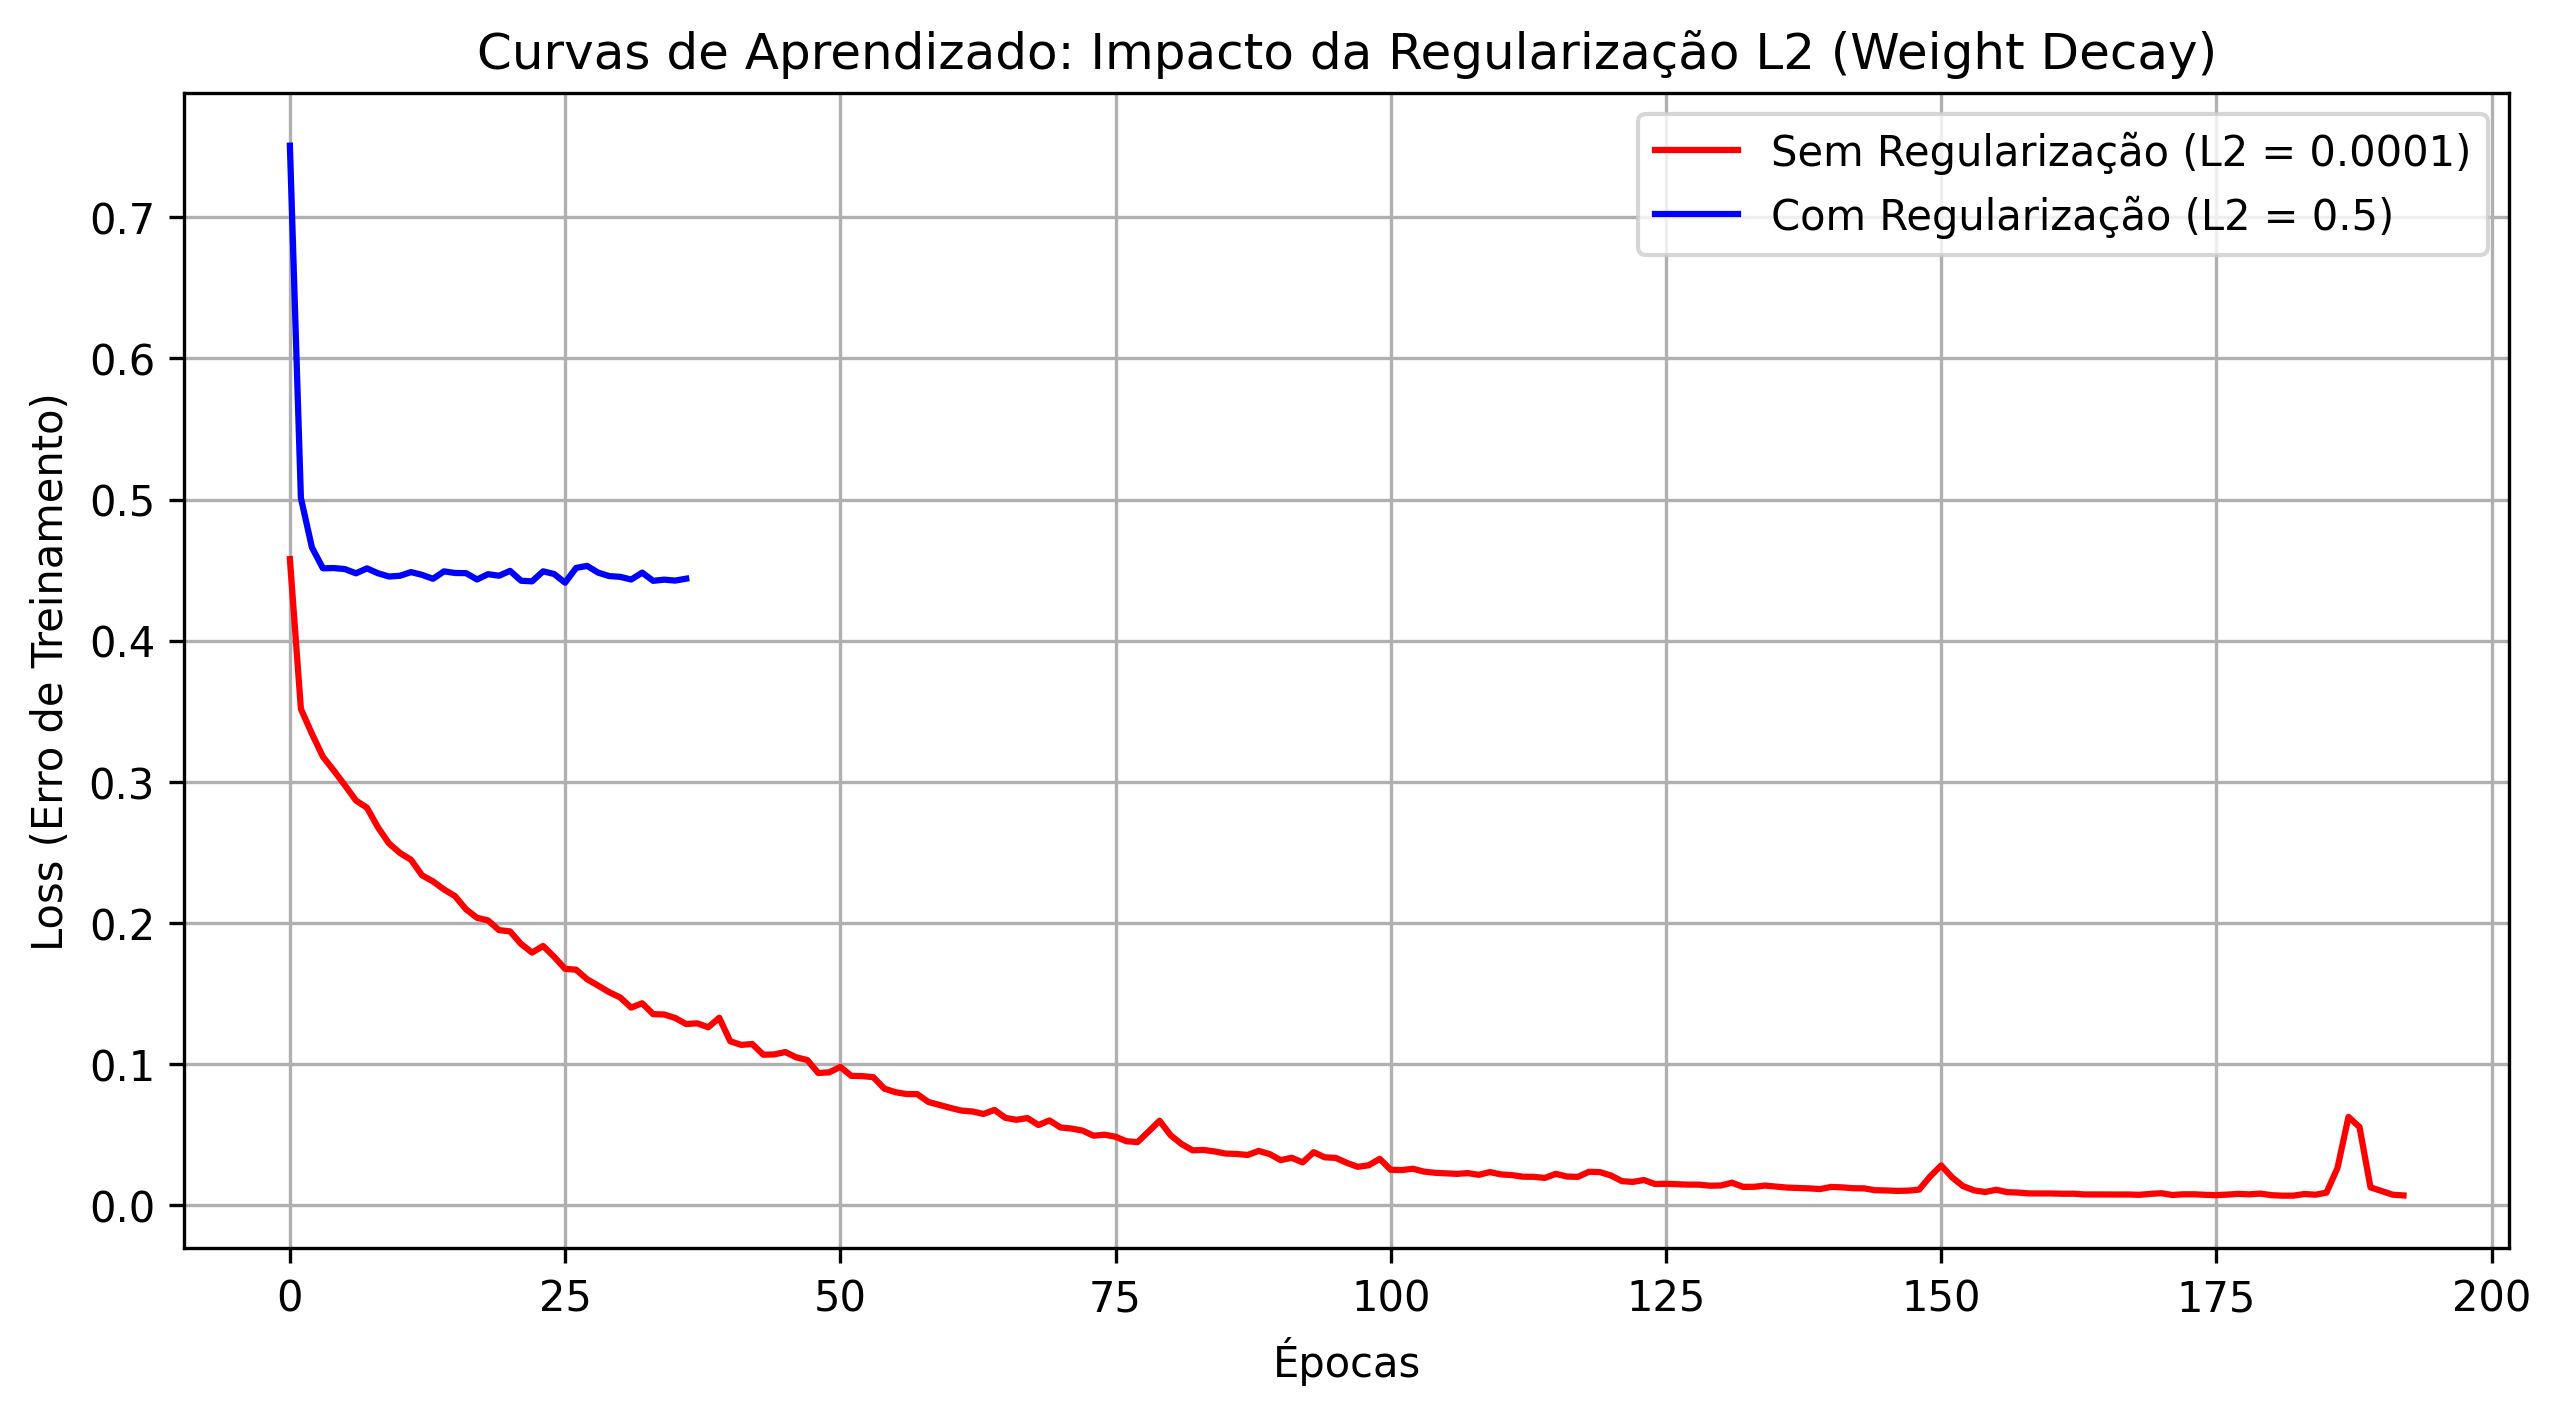
\includegraphics[width=0.8\textwidth]{grafico_regularizacao.png}
    \caption{Curvas de aprendizado mostrando o efeito das penalidades de Regularização L2 na redução do erro de treinamento.}
    \label{fig:regularizacao}
\end{figure}

\end{document}
